\documentclass[11pt]{article}
\usepackage{geometry}
\geometry{a4paper, margin=1in}
\usepackage{amsmath, amssymb}
\usepackage{graphicx}
\usepackage{xeCJK}
\setCJKmainfont{Noto Serif CJK SC}
\usepackage{booktabs}
\usepackage{hyperref}
\usepackage{float}
\usepackage{tikz}
\usepackage{pgfplots}


\begin{document}

\title{大语言模型在代码生成中的应用:挑战、技术、应用与未来}
\author{
    尹超 \\
    2023K8009926003 \\
    人工智能2023级 \\
}
\date{2025年5月}
\maketitle

\begin{abstract}
大语言模型(LLMs)通过自然语言处理技术,使用户能够以人类语言生成可执行代码,显著降低了编程门槛。本文探讨了LLMs在代码生成中的技术原理、面临的挑战、应用场景及未来发展趋势。基于可靠的学术论文和技术博客,我们分析了LLMs如何通过Transformer架构和大规模代码数据集实现代码生成,讨论了资源需求、代码错误、偏见和安全风险等挑战,并展示了其在代码补全、调试、翻译和低代码平台中的应用。未来,LLMs预计将通过改进训练方法和模型架构进一步提高准确性和安全性。本文通过数据和案例(如HumanEval和HumanEval+基准测试)以及多张图表(模型性能对比、错误类型分布、代码生成流程图、性能随时间改进)增强可读性,为研究者和开发者提供全面参考。
\end{abstract}

\section{引言}
大语言模型(LLMs)是基于深度学习的自然语言处理模型,能够理解和生成类人文本。近年来,LLMs在代码生成领域的应用显著增长,使非专业人士也能通过自然语言描述生成可执行代码。例如,GitHub Copilot通过理解用户输入的注释或代码片段,自动生成完整的函数实现,研究表明其可将数据预处理任务的耗时从小时缩短到分钟。% \cite{github_copilot_study})。
本文系统探讨LLMs在代码生成中的技术原理、挑战、应用场景及未来发展,基于可靠来源提供深入分析。

\subsection{LLMs的发展}
自2017年Transformer架构提出以来,% \cite{vaswani2017attention}),
LLMs经历了快速发展。早期模型如GPT-3拥有1750亿参数,而2024年的模型如Llama 3.1 405B进一步扩展了规模。这些模型通过在包含数十亿行代码的公开数据集(如GitHub代码库)上训练,展现出强大的代码生成能力。专门为代码生成设计的模型,如OpenAI的Codex和Meta的Code Llama,进一步优化了性能,使编程更加普及。

\section{技术原理}
\subsection{Transformer架构}
LLMs通常基于Transformer架构,这是一种通过自注意力机制捕捉序列数据关系的神经网络。% \cite{vaswani2017attention})。
Transformer由多个层组成,包括自注意力层、前馈层和归一化层,能够高效处理长序列数据。自注意力机制允许模型关注输入序列中的关键部分,从而理解复杂的代码结构。代码生成模型如Code Llama和Codex在训练时使用包含数十亿代码行的数据集,以学习编程语言的语法和语义。

\begin{figure}[H]
    \centering
    \href{https://papers.nips.cc/paper_files/paper/2017/file/3f5ee243547dee91fbd053c1c4a845aa-Paper.pdf}{%
        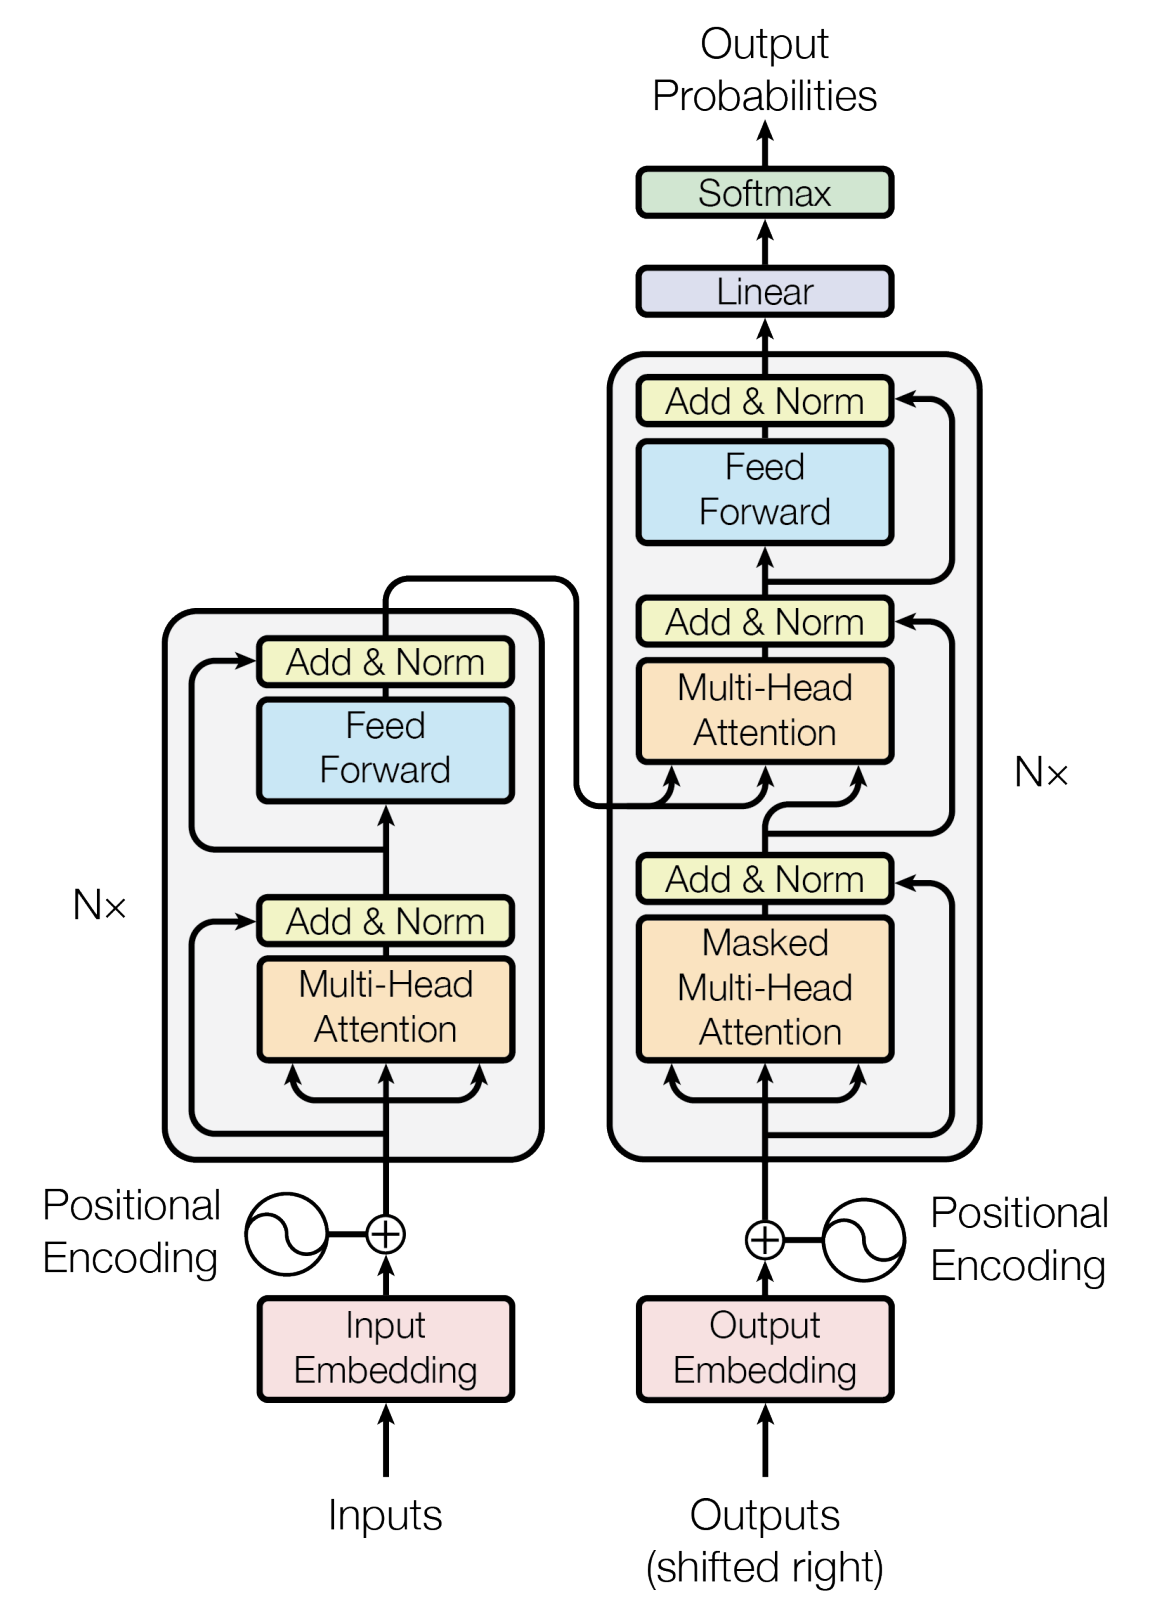
\includegraphics[width=0.8\textwidth]{transformer_architecture.png}%
    }
    \caption{\href{https://papers.nips.cc/paper_files/paper/2017/file/3f5ee243547dee91fbd053c1c4a845aa-Paper.pdf}{Transformer架构示意图}}%
    \label{fig:transformer}
\end{figure}

\subsection{代码生成流程}
LLMs生成代码的过程包括以下步骤:
\begin{enumerate}
    \item \textbf{理解提示}:分析用户输入的自然语言描述,提取意图和需求。例如,用户输入“写一个排序函数”,模型识别排序算法的需求。
    \item \textbf{检索模式}:从训练数据中检索相关代码模式,如快速排序或冒泡排序的实现。
    \item \textbf{组装片段}:将检索到的代码片段组合成连贯结构,确保语法正确。
    \item \textbf{生成代码}:输出符合语法的可执行代码,并根据上下文调整细节。
\end{enumerate}

\begin{figure}[H]
    \centering
    \href{https://mskadu.medium.com/generating-code-with-llms-a-developers-guide-part-1-0c381dc3e57a}{%
        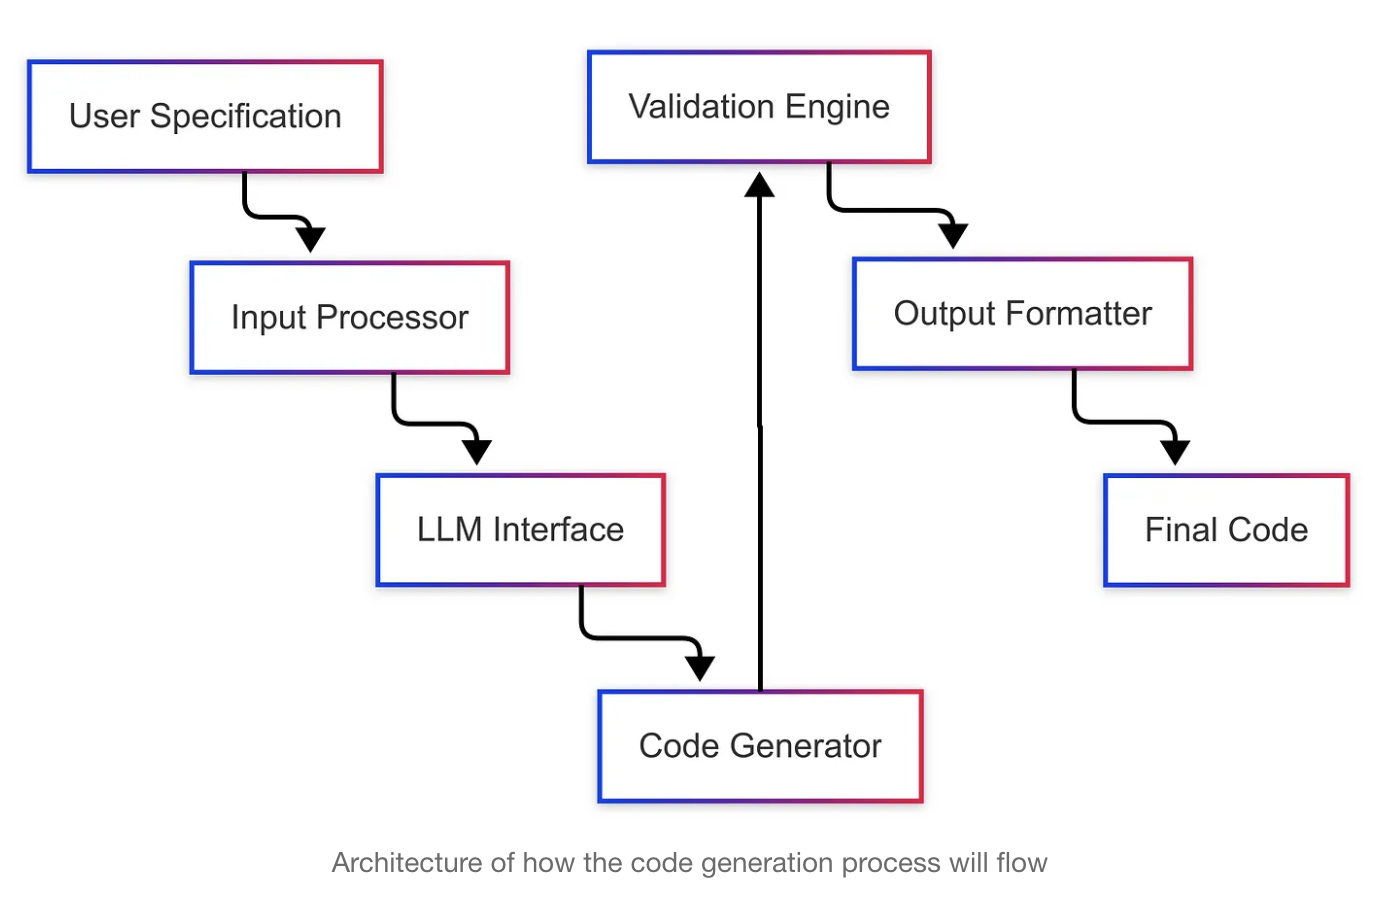
\includegraphics[width=0.8\textwidth]{code_generation_flowchart.png}%
    }
    \caption{\href{https://mskadu.medium.com/generating-code-with-llms-a-developers-guide-part-1-0c381dc3e57a}{大语言模型代码生成流程图}}
    \label{fig:flowchart}
\end{figure}

\section{挑战}
\subsection{资源需求}
训练LLMs需要大量计算资源。例如,Llama 3.1-8B模型需要700万GPU小时,而405B模型需要3100万GPU小时。% \cite{github_copilot_study})。
这不仅导致高昂的成本,还对环境造成影响,如碳排放问题。量化技术(如OmniQuant 4位量化,困惑度5.97)虽然降低了推理成本,但训练成本仍是中小型组织的障碍。

\subsection{语法与语义错误}
生成的代码常包含错误。研究显示,在557个代码片段中,约40\%存在语法错误,而在APPS+基准测试中,语义错误率超过50\%。% \cite{dou2024wrong})。
例如,ChatGPT生成的Java代码中有46.4\%存在非法索引错误。研究表明,功能性错误(Functional Bugs)占比最高,其次是运行时错误(Runtime Bugs),语法错误(Syntax Bugs)占比最低。图\ref{fig:error_types}展示了错误类型的分布。

\begin{figure}[H]
    \centering
    \href{https://arxiv.org/pdf/2407.06153}{%
        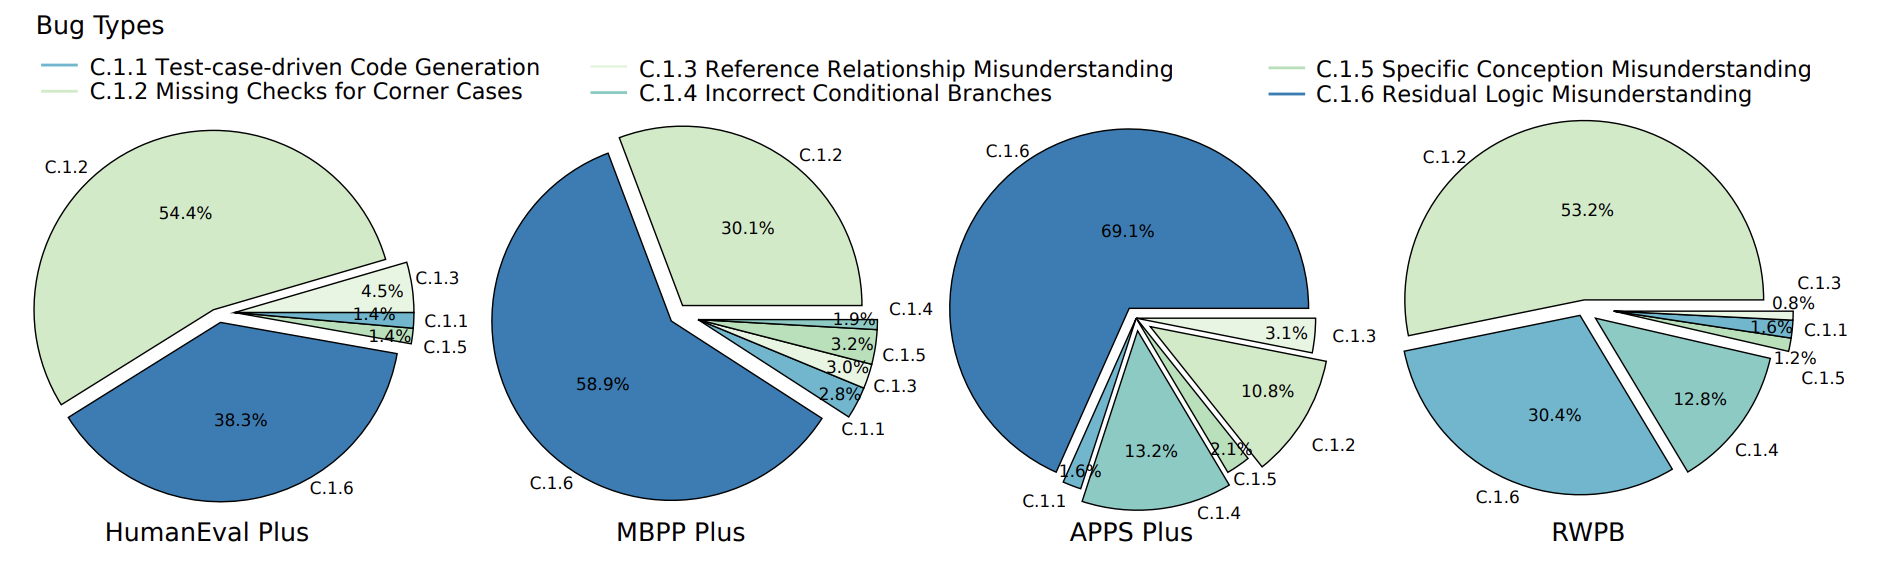
\includegraphics[width=0.9\textwidth]{error_types_pie.png}%
    }
    \caption{\href{https://arxiv.org/pdf/2407.06153}{LLM生成代码中错误类型的分布}}
    \label{fig:error_types}
\end{figure}

\subsection{偏见}
LLMs在多语言任务中表现出偏见。例如,中文指令下pass@1得分下降17.2\%,CodeLlama-34B在Java任务中下降37.8\%。% \cite{github_copilot_study})。
这可能源于训练数据中英语代码占主导地位。此外,社会偏见也存在,如Codex的CBS得分高达82.64\%,可能导致不公平的代码生成结果。

\subsection{安全风险}
LLMs生成的代码可能包含安全漏洞。研究表明,Copilot生成代码的40\%不安全,81\%的2049个代码库存在漏洞。% \cite{github_copilot_study})。
例如,生成的代码可能包含SQL注入或缓冲区溢出等问题,这对生产环境部署构成挑战。

\section{应用场景}
\subsection{代码生成与补全}
工具如GitHub Copilot和Code Llama广泛用于代码补全。Code Llama-34B在HumanEval上达到53.7\%的pass@1得分,与ChatGPT相当。% \cite{code_llama})。
根据GitHub的研究,使用Copilot的开发者完成任务的速度提高了55\%(1小时11分钟对比2小时41分钟),完成率为78\%,而未使用Copilot的开发者为70\%。% \cite{github_copilot_study})。
此外,73\%的开发者表示Copilot帮助他们保持专注,87\%认为它减少了重复任务的心理负担。

\subsection{高级代码生成与搜索}
AlphaCode在Codeforces竞赛中排名前54.3\%,解决34.2\%的CodeContests问题。% \cite{github_copilot_study})。
RepoRift在CodeSearchNet上实现78.2\%的Success@10得分,展示出强大的代码搜索能力。这些工具通过理解复杂需求生成高级代码,适用于编程竞赛和大型项目。

\subsection{调试与翻译}
GPT-4在LeetCode上成功率超过90\%,Codex修复Python错误的能力比Java高50\%。% \cite{github_copilot_study})。
Flourine在8160次翻译中实现47\%的准确率,支持跨语言代码转换,如将Python代码转换为Java。

\subsection{集成到开发工作流}
LLMs正被集成到各种开发工具中,如IDE、CI/CD管道等。例如,GitHub Copilot直接集成到Visual Studio Code中,提供实时代码建议。此外,LLMs被用于自动化测试、代码审查和文档生成。例如,LLMs可以生成测试用例或分析代码以检测潜在错误,从而提高开发效率。

\subsection{低代码平台}
LLMs也被集成到低代码平台中,使非专业开发者能够通过自然语言描述创建应用程序。例如,Low-code LLM框架允许用户通过图形界面与LLM交互,设计工作流而无需编写复杂提示。% \cite{low_code_llm})。
这为“公民开发者”提供了创建复杂应用的可能性,显著降低了技术门槛。

\section{未来发展趋势}
未来,LLMs在代码生成中的发展将集中在以下方面:
\begin{itemize}
    \item \textbf{提高准确性}:通过改进训练数据和模型架构减少错误和幻觉。%(\cite{dou2024wrong})。
    \item \textbf{增强上下文理解}:更好地理解代码库和开发者意图,特别是在复杂项目中。
    \item \textbf{实时反馈}:集成到开发环境中,提供即时错误检测和建议。
    \item \textbf{多语言支持}:提升对低资源语言的生成能力,减少偏见。
    \item \textbf{安全性改进}:开发更安全的代码生成方法,降低漏洞风险。
\end{itemize}
此外,专用LLMs(如针对金融或医疗领域的模型)和CI/CD管道的广泛集成将推动开发流程的自动化。新兴基准测试如BigCodeBench表明,顶级模型如GPT-4o在更复杂任务上的pass@1得分仅为61.1\%,显示出未来改进的空间。% \cite{bigcodebench})。

\section{数据与案例}
\subsection{基准测试概述}
HumanEval是评估代码生成模型的标准基准测试,包含164个编程问题,测试模型的函数正确性。% \cite{chen_2021})。
HumanEval+是其扩展版本,增加了更多测试用例以提供更严格的评估。% \cite{evalplus_leaderboard})。
此外,BigCodeBench等新兴基准测试通过更复杂的任务评估模型的实际编程能力。

\subsection{HumanEval基准测试}
以下是部分顶级模型在HumanEval上的pass@1得分:

\begin{table}[H]
    \centering
    \begin{tabular}{lc}
        \toprule
        模型 & Pass@1 (\%) \\
        \midrule
        O1 Preview & 92.4 \\
        GPT-4o & 90.2 \\
        Llama 3.1 405B & 89.0 \\
        Grok-2 & 88.4 \\
        Claude3 Opus & 84.9 \\
        \bottomrule
    \end{tabular}
    \caption{顶级LLMs在HumanEval上的pass@1得分}%(来源:\cite{bracai_humaneval})}
    \label{tab:humaneval}
\end{table}

\begin{figure}[H]
    \centering
    \href{https://www.bracai.eu/post/humaneval-benchmark}{%
    \begin{tikzpicture}
    \begin{axis}[
        ybar,
        width=0.8\textwidth,
        height=6cm,
        bar width=0.15cm,
        enlargelimits=0.15,
        ylabel={Pass@1 得分 (\%)},
        xlabel={模型},
        symbolic x coords={O1 Preview, GPT-4o, Llama 3.1 405B, Grok-2, Claude3 Opus},
        xtick=data,
        x tick label style={rotate=45, anchor=north east, inner sep=2pt},
        ymin=0, ymax=100,
        nodes near coords,
        nodes near coords style={font=\footnotesize},
        title={顶级 LLMs 在 HumanEval 上的 Pass@1 得分对比},
    ]
    \addplot coordinates {
        (O1 Preview, 92.4)
        (GPT-4o, 90.2)
        (Llama 3.1 405B, 89.0)
        (Grok-2, 88.4)
        (Claude3 Opus, 84.9)
    };
    \end{axis}
    \end{tikzpicture}
    }
    \caption{\href{https://www.bracai.eu/post/humaneval-benchmark}{顶级 LLMs 在 HumanEval 上的 Pass@1 得分对比(来源:BRACAI HumanEval Benchmark)}}
    \label{fig:humaneval_performance}
\end{figure}

\subsection{HumanEval+基准测试}
HumanEval+通过增加测试用例提高了评估难度。以下是部分模型在HumanEval+上的pass@1得分:

\begin{table}[H]
    \centering
    \begin{tabular}{lc}
        \toprule
        模型 & Pass@1 (\%) \\
        \midrule
        O1 Preview & 89.0 \\
        Qwen2.5-Coder-32B-Instruct & 87.2 \\
        GPT-4o & 87.2 \\
        DeepSeek-V3 & 86.6 \\
        Gemini 1.5 Pro & 79.3 \\
        \bottomrule
    \end{tabular}
    \caption{顶级LLMs在HumanEval+上的pass@1得分}%(来源:\cite{evalplus_leaderboard})}
    \label{tab:humaneval_plus}
\end{table}

\begin{figure}[H]
    \centering
    \href{https://arxiv.org/abs/2107.03374}{%
        \begin{tikzpicture}
        \begin{axis}[
            width=0.8\textwidth,
            height=6cm,
            xlabel={年份},
            ylabel={Pass@1 得分 (\%)},
            xtick={2021, 2023, 2024},
            ymin=0, ymax=100,
            grid=major,
            title={HumanEval 上 Pass@1 得分的随时间改进},
            nodes near coords,
            nodes near coords style={font=\footnotesize},
        ]
        \addplot[
            mark=*,
            blue,
            thick
        ] coordinates {
            (2021, 28.8)
            (2023, 67.0)
            (2024, 92.4)
        };
        \end{axis}
        \end{tikzpicture}
    }
    \caption{\href{https://arxiv.org/abs/2107.03374}{HumanEval 上 Pass@1 得分的随时间改进(来源:相关文献)}}
    \label{fig:performance_trend}
\end{figure}

\subsection{性能随时间改进}
自2021年HumanEval发布以来,LLMs在代码生成任务上的性能持续提升。图\ref{fig:performance_trend}展示了HumanEval上pass@1得分的随时间改进。

\begin{figure}[H]
    \centering
    \href{https://evalplus.github.io/leaderboard.html}{%
    \begin{tikzpicture}
    \begin{axis}[
        ybar,
        width=0.8\textwidth,
        height=6cm,
        bar width=0.15cm,
        enlargelimits=0.15,
        ylabel={Pass@1 得分 (\%)},
        xlabel={模型},
        xlabel style={yshift=-2cm},   % 向下移动 1cm
        symbolic x coords={O1 Preview, Qwen2.5-Coder, GPT-4o, DeepSeek-V3, Gemini 1.5 Pro},
        xtick=data,
        x tick label style={rotate=45, anchor=north east, inner sep=2pt},
        ymin=0, ymax=100,
        nodes near coords,
        nodes near coords style={font=\footnotesize},
        title={顶级 LLMs 在 HumanEval+ 上的 Pass@1 得分对比},
    ]
    \addplot coordinates {
        (O1 Preview, 89.0)
        (Qwen2.5-Coder, 87.2)
        (GPT-4o, 87.2)
        (DeepSeek-V3, 86.6)
        (Gemini 1.5 Pro, 79.3)
    };
    \end{axis}
    \end{tikzpicture}
    }
    \caption{\href{https://evalplus.github.io/leaderboard.html}{顶级 LLMs 在 HumanEval+ 上的 Pass@1 得分对比(来源:EvalPlus Leaderboard)}}
    \label{fig:humaneval_plus_performance}
\end{figure}

\section{结论}
大语言模型在代码生成领域的应用显著提高了开发效率,使非专业人士也能参与编程。然而,高资源需求、代码错误、偏见和安全风险仍是主要挑战。未来,通过改进训练方法、增强上下文理解和安全性,LLMs将在软件开发中发挥更大作用。

\section{参考文献}
\begin{itemize}
    \item \href{https://arxiv.org/abs/1706.03762}{Attention is All You Need - Vaswani et al.}
    \item \href{https://arxiv.org/abs/2407.06153}{What's Wrong with Your Code Generated by Large Language Models? - Dou et al.}
    \item \href{https://arxiv.org/abs/2304.08103}{Low-code LLM: Graphical User Interface over Large Language Models - Cai et al.}
    \item \href{https://arxiv.org/abs/2107.03374}{Evaluating Large Language Models Trained on Code - Chen et al.}
    \item \href{https://www.bracai.eu/post/humaneval-benchmark}{HumanEval Benchmark - BRACAI}
    \item \href{https://evalplus.github.io/leaderboard.html}{EvalPlus Leaderboard, HumanEval+ version 0.1.10}
    \item \href{https://github.blog/news-insights/research/research-quantifying-github-copilots-impact-on-developer-productivity-and-happiness/}{Research: Quantifying GitHub Copilot’s Impact on Developer Productivity and Happiness - GitHub Blog}
    \item \href{https://ai.meta.com/research/publications/code-llama-open-foundation-models-for-code/}{Code Llama: Open Foundation Models for Code - Meta AI}
    \item \href{https://huggingface.co/blog/leaderboard-bigcodebench}{BigCodeBench: The Next Generation of HumanEval - Hugging Face Blog}
\end{itemize}

\end{document}